% This is samplepaper.tex, a sample chapter demonstrating the
% LLNCS macro package for Springer Computer Science proceedings;
% Version 2.20 of 2017/10/04
%
\documentclass[runningheads]{llncs}
%
\usepackage{xcolor}


\usepackage{graphicx}


\usepackage[utf8]{inputenc} %Together with 'spanish' package, allows you to write accents 

%This package allows the use of accents, the parameter 'es-tabla' writes Tabla instead of 'Cuadro', the parameter es-noindentfirst makes that the first line after each section and subsection is not indented
\usepackage[spanish,activeacute,es-tabla,es-noindentfirst]{babel}

%This package allows you among other things, use as option [H] in tables and figures, which set the object just where you put in the source code.
\usepackage{float}

%This package allows you to write pseudocode, you should read the docummentation to use it properly 
\usepackage{algorithm2e}

%Packages to write math
\usepackage{amssymb}
\usepackage{amsmath}

%permite el formato de múltiple citación agrupada dentro de los corchetes
\usepackage{cite} 

\usepackage{times}
\usepackage{color}

%Package that help to write text that will appear like you write in the final documment
\usepackage{verbatim}

%This package allows you to configure tables and figures
\usepackage{caption}

%Package to customize formats to the tables
\usepackage{booktabs}

%Package to control hiperlinks
\usepackage[breaklinks=true]{hyperref}
\hypersetup{
	colorlinks=true,
	linkcolor=blue,
	filecolor=magenta,      
	urlcolor=blue,
	citecolor=cyan,
}

%Package to stablish the margins of the documment
\usepackage{vmargin}

%A0, A1, ..., A9, B0, B1, ..., B9, C0, ..., C9, USletter, USlegal, and USexecutive
\setpapersize{A4}
%\setmarginsrb{hleftmargini}{htopmargini}{hrightmargini}{hbottommargini}%
%{hheadheighti}{hheadsepi}{hfootheighti}{hfootskipi}

\setmarginsrb{30mm}{25mm}{30mm}{25mm}{6mm}{7mm}{5mm}{15mm}

%También puede utilizar esta sintaxis para establcer los márgenes con el paquete {vmargin}
%\setmargins{3.0cm}       % margen izquierdo
%{1.5cm}                        % margen superior
%{14.5cm}                      % anchura del texto
%{23.42cm}                    % altura del texto
%{10pt}                           % altura de los encabezados
%{1cm}                           % espacio entre el texto y los encabezados
%{0pt}                             % altura del pie de página
%{2cm}         

%Estos paquetes se utilian para escribir psudocódigo, sin embargo en estos momentos se está utilizando el paquete {algorithm2e}
%\usepackage{algpseudocode}
%\usepackage{algorithmicx}
%\usepackage{algorithm}

\definecolor{gray97}{gray}{.97}
\definecolor{gray75}{gray}{.75}
\definecolor{gray45}{gray}{.45}

%Packages to write code in various programming languajes, please, see the docummentation 
\usepackage{listings}
\usepackage{listingsutf8}
\lstset{frame=Ltb,
	framerule=0pt,
	aboveskip=0.5cm,
	framextopmargin=3pt,
	framexbottommargin=3pt,
	framexleftmargin=0.4cm,
	framesep=0pt,
	rulesep=.4pt,
	backgroundcolor=\color{gray97},
	rulesepcolor=\color{black},
	%
	stringstyle=\ttfamily,
	showstringspaces = false,
	basicstyle=\small\ttfamily,
	commentstyle=\color{blue},
	keywordstyle=\bfseries,
	%
	numbers=left,
	numbersep=15pt,
	numberstyle=\tiny,
	numberfirstline = false,
	breaklines=true,
}
\lstnewenvironment{listing}[1][]
{\lstset{#1}\pagebreak[0]}{\pagebreak[0]}

\lstdefinestyle{consola}
{basicstyle=\scriptsize\bf\ttfamily,
	backgroundcolor=\color{gray75},
}
\lstdefinestyle{C}
{language=C,
}
% Used for displaying a sample figure. If possible, figure files should
% be included in EPS format.
%
% If you use the hyperref package, please uncomment the following line
% to display URLs in blue roman font according to Springer's eBook style:
\renewcommand\UrlFont{\color{blue}\rmfamily}

%\renewcommand\Algorithmname{Algoritmo}
\renewcommand\examplename{Ejemplo}
\renewcommand\exercisename{Ejercicio}
\renewcommand\figurename{Fig.}
\renewcommand\keywordname{{\bf T\'erminos Clave:}}
\renewcommand\indexname{Index}
\renewcommand\lemmaname{Lema}
\renewcommand\contriblistname{Lista de colaboradores}
\renewcommand\listfigurename{Lista de Figuras}
\renewcommand\listtablename{Lista of Tablas}
\renewcommand\mailname{{\it Correspondencia para\/}:}
\renewcommand\noteaddname{Note added in proof}
\renewcommand\notename{Nota}
\renewcommand\partname{Parte}
\renewcommand\problemname{Problema}
\renewcommand\proofname{Demostración}
\renewcommand\propertyname{Propiedad}
\renewcommand\propositionname{Proposici\'on}
\renewcommand\questionname{Pregunta}
\renewcommand\remarkname{Remark}
\renewcommand\seename{Ver}
\renewcommand\solutionname{Soluci\'on}
\renewcommand\theoremname{Teorema}
\begin{document}

\title{Creacion de Sistema de Gestion de Colportaje}
%
%\titlerunning{Abbreviated paper title}
% If the paper title is too long for the running head, you can set
% an abbreviated paper title here
%
\author{Ismael Alejandro Flamenco Rosales\inst{1}}
%
\authorrunning{LNCS traducido y editado por \emph{Lafhart}.}
% First names are abbreviated in the running head.
% If there are more than two authors, 'et al.' is used.
%
\institute{Universidad Linda Vista, Ex-Finca Santa Cruz \# 1, 29750\\
\email{fdi@ulv.edu.mx}\\
\url{http://www.ulv.edu.mx/fdi}\\
\email{ismael.flamenco@ulv.edu.mx}
}

\maketitle

\newpage

\section{\centering{Generalidades del Proyecto}}



\subsection{Antecedentes}
La Universidad Linda Vista, cuenta con un grupo de alumnos que financia sus estudios a traves de la venta de publicaciones llamado colportaje, los alumnos salen cada periodo vacacional de invierno y verano a diversos estados de Mexico o el extranjero. El alumno realiza la compra de las publicaciones a la casa editora GEMA, y realiza la venta minorista de manera directa con el cliente, este proceso se realiza a traves de un talonario impreso en papel, en el cual, se registra la informacion de la venta, que consiste entre otros titulo del libro, precio, fecha de entrega y fechas de pago por parte del cliente, etc. Terminada la fase anterior se emite una copia del talonario al cliente y el recibo original queda a resguardo del colportor, para el control de ventas.
Actualmente, no se cuenta con ninguna otra herramienta creada o emitida por la casa editora o por la universidad que permita registrar la informacion comentada anteriormente a traves de una aplicacion que este enfocada a la gestion del colportaje, sin embargo ha sido de interes por parte de los alumnos que esta exista, en virtud de lo manifestado en el cuestionario aplicado a una muestra de 35 colportores universitarios de edades entre los 18 a los 30 años, con el objetivo de obtener información sobre cómo realizan su trabajo y cómo llevan el control de sus ventas, compras y créditos. Los resultados de la encuesta ayudaron a comprender los desafíos y obstáculos que enfrentan los colportores en su trabajo diario y pueden ser utilizados para desarrollar soluciones que los apoyen a gestionar la informacion de ventas de manera digital.

\subsection{Descripción de la empresa}

La Universidad Linda Vista apoya y motiva al estudiante para ser un colportor y financiar de esta manera sus estudios a traves del club KERUSSO S.C. Esta se encuentra ubicada en las instalaciones de la misma universidad con direccion en Ex-Finca Santa Cruz \# 1, 29750 Municipio de Pueblo Nuevo Solistahuacán, Chiapas, Mexico. Este club dispone con una organización interna conformada por estudiantes y empleados y tiene como porposito capacitar a los estudiantes para tener exito en el colportaje, brindandoles herramientas necesarias para ser efectivos en su campo correspondiente.\\
Este club cuenta con una oficina cuya informacion de contacto es la siguiente: Telefono (+52) 961 304 8241 y correo electronico colportores.kerusso@ulv.edu.mx.

\subsection*{Filosofía:}
\begin{itemize}
    \item De nuestros libros y periódicos han de emanar brillantes rayos de luz que han de iluminar al mundo con respecto a la verdad presente.
    \item El Señor ha instituido un plan por el cual muchos alumnos de nuestros colegios pueden aprender lecciones prácticas necesarias para tener éxito en la vida posterior.
    \item Cuando finalizan las clases, habrá oportunidades para que muchos salgan al campo como Colportores evangélicos.
\end{itemize}
\subsection*{Misión: }
Instruir a estudiantes bajo la dirección de Dios, como un ministerio colaborador en el proceso educativo de todo joven.
\subsection*{Visión: }
Distribuir el mensaje de salvación a través de publicaciones adventistas, con jóvenes capaces y dispuestos a alcanzar almas para Cristo en todo México.
\subsection*{Blanco: }
Proclamando las Verdades del Evangelio con las publicaciones hasta que Cristo venga.
\subsection*{Lema: }
Motivados por el Espíritu Santo.
\subsection*{Voto:} 
Colportores estudiantes, unidos por el compromiso de servir a la sociedad, llevando el mensaje de salvación a través de la página impresa.
\subsubsection*{Valores: }
\begin{itemize}
    \item Integridad
    \item Consagración
    \item Fidelidad
    \item Trabajo
    \item Responsabilidad
    \item Lealtad
    \item Liderazgo
\end{itemize}

\subsection{Organizacion  de la Empresa}
\begin{figure}[H]
	\centering\captionsetup{width=0.8\textwidth}
	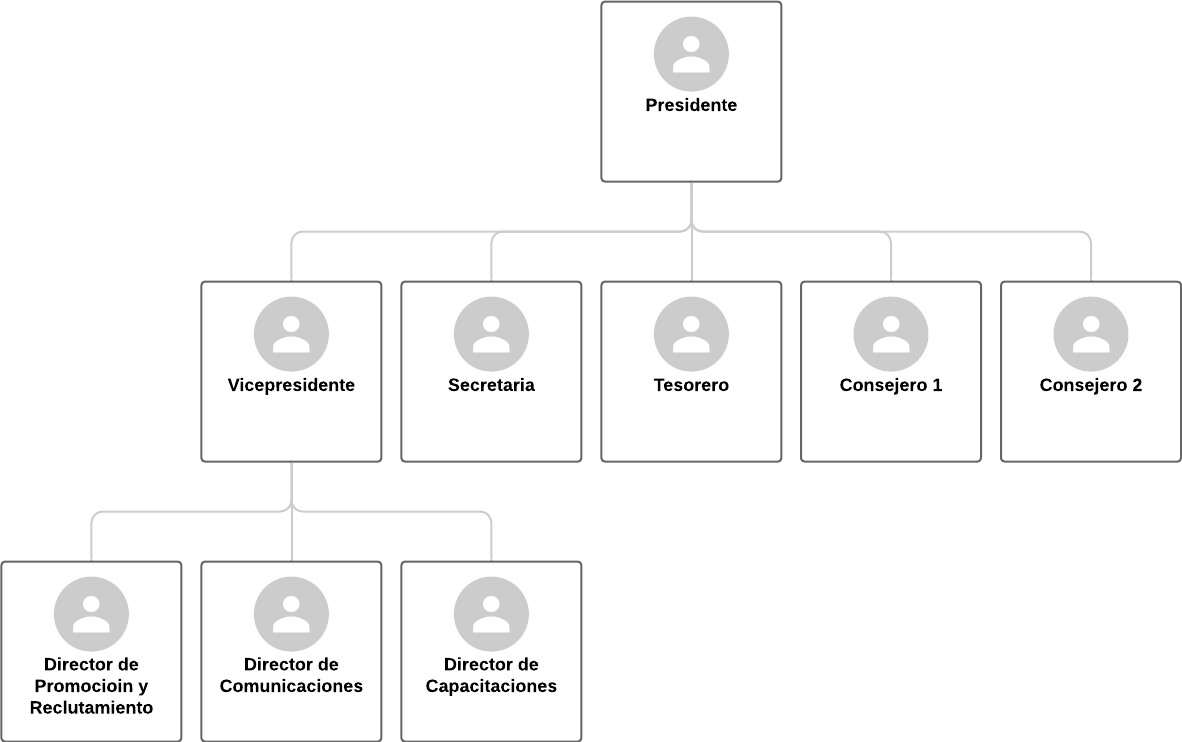
\includegraphics[width=1\textwidth]{figures/Organigrama.png}
	\caption{Organizacion Empresarial de Kerusso} \label{fig1}
\end{figure}


\subsection{Plantemiento del Problema}
Actualmente el club de colportores KERUSSO, gestiona sus ventas por medio de talonarios físicos como ya se ha mencionado, este sistema si bien es efectivo y funcional, es un sistema que tiene muchos inconvenientes para los colportores, tales como:
\begin{itemize}
    \item Acumulación de recibos por cada pedido complicando la gestión de las ventas y pedidos. 
    \item Riesgo de extravio de los recibos, en virtud de no existir un respaldo de esta información.
    \item La gestión de cobros y pedidos se hace compleja y tediosa.
    \item No existe un sistema que notifique al colportor sobre la fecha de entrega y cobro de los materiales, existiendo retrasos en la entrega del pedido y del cobro del producto por parte del colportor.
\end{itemize}
En vista de lo anterior, se ha identificado una necesidad por parte de los colportores y el club KERUSSO, de crear una herramienta que optimice los procesos, disponiendo de una alternativa para una mejor gestión del colportaje, haciendo uso de las tecnologías de la informacion.

\subsection{Objetivos del Proyecto}
\subsection*{Objetivo General}
Desarrollar un software que permita optimizar los procesos de gestion del colportaje de los estudiantes del club de colportores Kerusso.
\subsection*{Objetivos Especificos}
\begin{itemize}
    \item Obtener y analizar los requerimientos para el desarrollo del software.
    \item Diseñar las interfaces graficas y logicas del software.
    \item Codificar los modulos del software de acuerdo a los requerimientos y diseños.
    \item Realizar pruebas funcionales y de calidad de software.
    \item Implementar el software para su produccion.
    \item Capacitar a los usuarios finales en el uso del software.
\end{itemize}

\subsection{Justificacion}

La constante necesidad de estar actualizados con las tecnologías actuales y aprovechar esos recursos es algo fundamental actualmente para obetener el mayor rendimiento y optimización en nuestro trabajo. Es por eso que, con base en las respuestas del cuestionario y las problemáticas mencionadas anteriormente, se observa la necesidad de desarrollar un sistema para mejorar el proceso de gestión de ventas y pedidos en el colportaje estudiantil. Por lo tanto, se propone la creacion e implementación de una herramienta digital de gestión de ventas y pedidos para los colportores. Al realizar este sistema, el colportor se vera beneficiado en una menor inversion de tiempo en el registro y control de ventas y pedidos asi como una reduccion de uso de papel y brindar una mejor experiencia de colportaje. A partir de este sistema, podrian desarrollarse herramientas que beneficien y mejoren la supervicion y consulta de ventas por parte de los colportores de manera centralizada y contar con informacion que permita tomar desiciones para futuras campañas de colportaje desde la directiva del club Kerusso.


\subsection{Alcances y Limitaciones}
El sistema de gestión de colportaje permitirá controlar las ventas, pedidos, clientes, creditos y catalogo de libros disponibles, y como una primera implementacion de este, se limitara a la informacion que dispone el club de colportores Kerusso. Además, el colportor asociado podrá supervisar y consultar las ventas de sus colportores asignados.

\newpage

\section{\centering{Marco Teorico}}

\subsection{Conceptos Financieros}
\subsubsection{Compra de libros a credito: }Esta es una forma de adquirir libros en la que el colportor puede recibir los libros y pagarlos en los términos y plazos acordados. Es similar a un préstamo que se devuelve en un tiempo determinado. Esta modalidad de compra facilita la adquisición de materiales y permite que el colportor pueda ofrecer más opciones a los clientes. Además, es una forma de trabajo para aquellos colportores que no cuentan con los recursos necesarios para adquirir los libros de manera inmediata.

\subsubsection{Compra de libros a contado: }Es la forma de adquirir libros pagando su precio total en el momento de la compra. Es decir, el colportor paga el precio total de los libros en el momento de adquirirlos en la editorial. Esta modalidad es ideal para aquellos que desean adquirir los materiales de manera inmediata y cuentan con los recursos necesarios. Además, permite que el colportor tenga un mayor control sobre sus ingresos y su flujo de efectivo.

\subsubsection{Venta a credito: }Es una modalidad en la que el colportor vende los libros a un cliente y acuerda un plazo para recibir el pago. El cliente puede pagar en cuotas y fechas acordadas previamente. Esta modalidad de venta es ideal para aquellos clientes que desean adquirir los materiales pero no cuentan con los recursos necesarios en ese momento o desean hacerlo en una cierta cantidad de pagos. Además, es una forma de fidelizar a los clientes y establecer una relación de confianza con ellos.

\subsubsection{Venta a contado: }Es otra forma de vender libros en la que el colportor recibe el pago total en el momento de la venta. Esta modalidad es ideal para aquellos clientes que desean adquirir los materiales de manera inmediata y si cuentan con los recursos necesarios. 

\subsubsection{Talonario: }Es un libro con una serie de cheques o comprobantes de pago que se utilizan para registrar las ventas y los pagos en el colportaje estudiantil adventista. El talonario es una herramienta fundamental para llevar un registro de las transacciones realizadas por el colportor y mantener un control eficiente de los pagos y las ventas. Además, permite que el colportor tenga una mayor organización y un mayor control sobre sus finanzas.

\subsubsection{Diezmo: }Es un compromiso que los colportores realizan con Dios y la iglesia adventista del séptimo día, designando un 10\% de las ganancias del colportaje como diezmo y entregándolo a la Asociación del campo al cual esta asignado el colportor. Esta contribución es una muestra de agradecimiento y compromiso con Dios, su iglesia y la labor que esta realiza. 

\subsubsection{Inventario de libros: }Es un registro donde se lleva un control exhaustivo de los libros y otros materiales que se tienen disponibles para la venta. Es importante tener un inventario actualizado para saber qué libros se tienen y cuáles se necesitan adquirir. El inventario permite optimizar el proceso de venta y asegurar la disponibilidad de los materiales para los clientes. Además, permite que el colportor tenga una mayor organización y un mayor control sobre sus ventas.

\subsubsection{Catálogo de precios: }Es una lista detallada de los materiales, su descripción, su precio segun el tipo de compra y venta. Esta herramienta permite que los colportores tengan una mayor eficiencia en su trabajo y puedan ofrecer a los clientes una amplia variedad de opciones y precios. Además, el catálogo de precios es una forma de mantener un control eficiente sobre los materiales disponibles y su precio, lo que permite una mejor toma de decisiones en cuanto a la adquisición y venta de materiales.



\subsection{Gestion de Proyectos}
La gestión de proyectos es una disciplina que implica la planificación, organización, dirección y control de los recursos (humanos, financieros, materiales) de un proyecto con el objetivo de alcanzar los objetivos establecidos en el tiempo, costo y calidad planificados. La gestión de proyectos implica la aplicación de conocimientos, habilidades, herramientas y técnicas para satisfacer los requisitos del proyecto como por ejemplo las metodologias de desarrollo \cite{Cita1}.

En el contexto del desarrollo de software, la gestión de proyectos implica la planificación, el seguimiento y el control de las actividades necesarias para crear software. Las metodologías de desarrollo de software son enfoques sistemáticos utilizados para organizar y controlar el proceso de desarrollo de software \cite{Cita2}. Algunas metodologías comunes de desarrollo de software incluyen el modelo en cascada, el modelo en espiral, el modelo ágil y el modelo DevOps. Cada metodología tiene sus propias ventajas y desventajas, y la elección de la metodología adecuada dependerá de los requisitos y limitaciones específicos del proyecto.

El ciclo de vida del software es el proceso de desarrollo de software que comienza desde la concepción del software hasta su retiro del mercado. El ciclo de vida del software se divide en varias fases, que incluyen el análisis de requisitos, el diseño, la construccion e implementación, las pruebas, el despliegue y el mantenimiento \cite{Cita3}. Cada fase del ciclo de vida del software tiene sus propios entregables y objetivos específicos, y el proceso de gestión de proyectos se aplica en cada una de estas fases para garantizar el éxito del proyecto.

\subsection{Desarrollo de Aplicaciones Móviles}
El desarrollo de aplicaciones móviles es el proceso de creación de aplicaciones informáticas diseñadas para ser utilizadas en dispositivos móviles. Implica la creación de software que se ejecute en sistemas operativos móviles, como Android o iOS, y comienza con la identificación de los requisitos de la aplicación y el diseño de la interfaz de usuario, integración de funcionalidades y algoritmos necesarios para su correcto funcionamiento. Después de la fase de desarrollo, se lleva a cabo un proceso de pruebas para garantizar su correcto funcionamiento en diferentes dispositivos móviles y sistemas operativos \cite{Cita4}.
Debido a la importancia de los dispositivos móviles en la vida cotidiana de muchas personas, el desarrollo de aplicaciones móviles es una actividad crítica en el mercado actual, ya que las aplicaciones móviles se utilizan para una amplia gama de actividades y su desarrollo adecuado es esencial para garantizar la satisfacción del usuario y el éxito de la aplicación \cite{Cita5}.


El diseño UI (User Interface) y UX (User Experience) son dos conceptos fundamentales en el desarrollo de aplicaciones móviles. La UI (User Interface) y la UX (User Experience) son dos disciplinas del diseño centradas en la creación de productos digitales enfocados en el usuario. La UI se enfoca en el diseño y la apariencia visual de una interfaz digital, incluyendo elementos como la disposición de los botones, la tipografía, los colores y los gráficos. Por otro lado, la UX se enfoca en la experiencia general del usuario al interactuar con un producto digital, considerando aspectos como la facilidad de uso, la eficiencia, la satisfacción y la accesibilidad \cite{Cita6}. Ambas disciplinas son esenciales para el desarrollo de productos digitales exitosos y su combinación adecuada puede llevar a una experiencia de usuario satisfactoria y una interfaz digital intuitiva. 

Para implementar el diseño UI / UX se utilizan herramientas como Adobe XD y Sketch, que permiten la creación de prototipos y diseños de interfaces gráficas. Además, se llevan a cabo pruebas de usabilidad y accesibilidad para asegurar que la aplicación móvil sea fácil de usar y accesible para todos los usuarios.

Los lenguajes de programación, como Swift, Java y Kotlin, son utilizados para desarrollar aplicaciones móviles para iOS y Android. Los desarrolladores deben tener un conocimiento sólido de estos lenguajes de programación y sus características para desarrollar aplicaciones móviles eficientes y escalables. Los lenguajes de programación específicos para cada plataforma, son necesarios para desarrollar aplicaciones nativas, aunque existen alternativas como las aplicaciones hibridas que permiten crear aplicaciones multiplataforma con una misma base de codigo utilizando frameworks como por ejemplo Flutter o React Native \cite{Cita7}.

Los frameworks son herramientas que permiten a los desarrolladores crear aplicaciones de manera más rápida y eficiente al proporcionar una estructura y conjunto de herramientas predefinidas \cite{Cita8}. 

\subsection{Diseño de Arquitectura}
La arquitectura de software es el conjunto de decisiones y soluciones adoptadas en el diseño y desarrollo de sistemas de software. Se enfoca en la estructura y organización de los componentes del sistema, así como las interacciones entre ellos y su comportamiento en tiempo de ejecución \cite{Cita9}.

El diseño de arquitectura de software es el proceso de definir la estructura, componentes, módulos, interfaces y otras características de un sistema de software, con el fin de satisfacer los requerimientos funcionales y no funcionales \cite{Cita9,Cita11}. Es un proceso que implica la creación de una estructura lógica y coherente para el software y es importante en el desarrollo de aplicaciones móviles, ya que ayuda a garantizar que las aplicaciones sean escalables y fáciles de mantener.

Los patrones de arquitectura de software son soluciones reutilizables a problemas comunes en el diseño y desarrollo de sistemas de software. Son modelos probados y documentados que pueden ser aplicados a diferentes contextos y problemas. Los patrones de arquitectura, como MVC, MVP y MVVM, son comúnmente utilizados en el desarrollo de aplicaciones móviles \cite{Cita11}. 

\subsection{Bases de de Datos}
Una base de datos es un conjunto de datos organizados y estructurados en un sistema de almacenamiento que permite acceder a la información y manipularla de manera eficiente y segura. Existen dos tipos principales de bases de datos: las bases de datos relacionales y las no relacionales. Una base de datos relacional es un tipo de sistema de almacenamiento de datos que utiliza tablas para organizar la información. Las tablas están compuestas por filas y columnas, donde cada columna representa un atributo o campo de la información y cada fila representa un registro o instancia de la información. Una base de datos no relacional es un tipo de sistema de almacenamiento de datos que no utiliza tablas relacionales para organizar la información. En su lugar, utiliza otras estructuras de datos, como grafos o documentos, para almacenar la información \cite{Cita12}.

La arquitectura de bases de datos se refiere a la estructura y organización de los componentes de un sistema de bases de datos, incluyendo la gestión de datos, el almacenamiento, la recuperación y el procesamiento de la información. La creación y administración de bases de datos es fundamental en el desarrollo de software, estas son utilizadas para almacenar y gestionar datos de manera organizada. Los desarrolladores también tienen en cuenta el diseño de la arquitectura de la base de datos, ya que esto ayuda a garantizar que sea escalable y fácil de mantener. El diseño de datos es un proceso que implica la creación de una estructura lógica y coherente para la información que se almacenará en la base de datos \cite{Cita13}. 

Las bases de datos se almacenan en servidores que permiten gestionar y acceder a grandes cantidades de información de manera eficiente y segura. Estos servidores pueden ser instalados de manera local o en la nube, y pueden ser accedidos por múltiples usuarios o aplicaciones simultáneamente. Este proporciona servicios de gestión de transacciones, seguridad, escalabilidad y disponibilidad para las aplicaciones que utilizan la base de datos. Los desarrolladores deben tener un conocimiento sólido de la administración y creación de servidores para garantizar que la base de datos sea accesible y segura. Pueden ser administrados mediante herramientas como cPanel y phpMyAdmin o cualquier administrador o gestor de bases de datos disponible y compatible, y pueden ser creados en plataformas en la nube como Amazon Web Services o Microsoft Azure \cite{Cita14}.


\subsection{Microservicios y API’s}
Los microservicios son una arquitectura de software que se enfoca en la creación de aplicaciones compuestas por servicios independientes y altamente cohesionados, que se comunican entre sí mediante interfaces bien definidas. Los microservicios ayudan a modularizar el software, lo que facilita la escalabilidad y el mantenimiento de los servicios individuales \cite{Cita15}.

Una API (Application Programming Interface) es un conjunto de funciones y protocolos que permiten la interacción entre diferentes componentes de software, como aplicaciones y servicios web, de manera estandarizada y segura. Las API’s proporcionan una interfaz de programación para que los desarrolladores puedan acceder a los microservicios y otros sistemas \cite{Cita16}.

 Los desarrolladores utilizan patrones de diseño, como el patrón de arquitectura de microservicios, para crear servicios que sean independientes y fáciles de mantener, ademas permiten una mayor flexibilidad en la gestión de recursos y en la implementación de actualizaciones .

\subsection{Aplicaciones en este proyecto}

En este proyecto se utiliza la metodología de desarrollo incremental, aplicada dentro de cada etapa del Ciclo de Vida del Software, que comprende las fases antes mencionadas. Para implementar esta metodología se utilizan herramientas de gestión de proyectos, como Trello y Notion, que permiten la asignación de tareas, seguimiento de avances y control de tiempos. Además, esto permite establecer reuniones de seguimiento para asegurar el cumplimiento de los objetivos establecidos y hacer una revisión de avances con el cliente.

El lenguaje de programación utilizado en este proyecto es Dart, que es un lenguaje de programación orientado a objetos y desarrollado por Google. Dart se utiliza principalmente para la creación de aplicaciones móviles con Flutter, pero también puede utilizarse para la creación de aplicaciones web y de escritorio. 

Ademas, se utilizan dos frameworks principales: Flutter para el desarrollo de la aplicación móvil y NodeJS para el desarrollo del backend y la creación de API's y microservicios. Para implementar los frameworks se utilizarán las respectivas herramientas de desarrollo, como Android Studio y Visual Studio Code para Flutter y Express para NodeJS. 

Para la arquitectura del software, se utilizarán patrones como MVVM y microservicios para crear una arquitectura escalable y fácilmente mantenible. Para implementar el diseño de arquitectura se utilizan herramientas como diagramas de flujo, y la arquitectura C4 para modelar y definir la estructura de la aplicacion.

Dentro del contexto de bases de datos, se utilizarán dos tipos de bases de datos: SQLite para el almacenamiento local de datos en la aplicación móvil ya que es una biblioteca de software que proporciona un sistema de gestión de bases de datos relacionales \cite{Cita17}, y MongoDB para el almacenamiento de datos del backend en la nube el cual es un sistema de base de datos no relacional de código abierto, que utiliza documentos JSON para almacenar y recuperar información \cite{Cita18}. A fin de gestionar las bases de datos de manera local, se utilizarán herramientas como MongoDB Compass que es una herramienta gráfica de administración y visualización de bases de datos MongoDB, que permite la exploración y manipulación de los datos de manera intuitiva y eficiente y SQLite Studio el cual es el gestor de bases de datos para SQLite.

Adicional a esto se usaran servicios de alojamiento de proveedores en la nube como MongoDB Atlas y SQLite Studio para el alojamiento local. Para implementar la administración y creación de servidores se utilizarán las respectivas herramientas de los proveedores elegidos.

\bibliographystyle{splncs04}
\bibliography{formato-fdi/bib/isma}

\end{document}
